\documentclass{standalone}
\usepackage{tikz-network}
\begin{document}
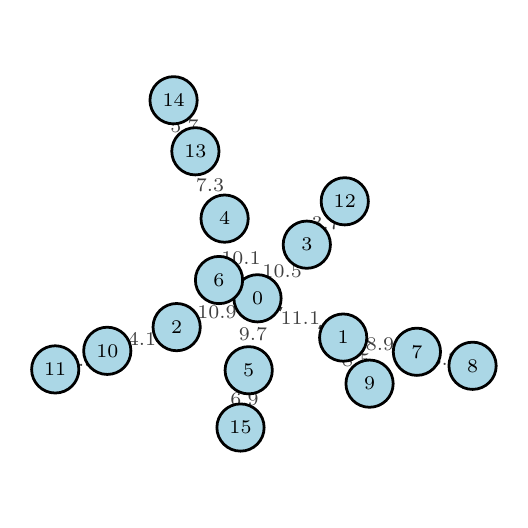
\begin{tikzpicture}
\clip (0,0) rectangle (6,6);
\Vertex[x=2.919,y=2.563,label=0]{0}
\Vertex[x=4.007,y=2.064,label=1]{1}
\Vertex[x=1.892,y=2.197,label=2]{2}
\Vertex[x=3.545,y=3.244,label=3]{3}
\Vertex[x=2.501,y=3.575,label=4]{4}
\Vertex[x=2.807,y=1.649,label=5]{5}
\Vertex[x=2.430,y=2.795,label=6]{6}
\Vertex[x=4.943,y=1.884,label=7]{7}
\Vertex[x=5.650,y=1.706,label=8]{8}
\Vertex[x=4.342,y=1.479,label=9]{9}
\Vertex[x=1.011,y=1.896,label=10]{10}
\Vertex[x=0.350,y=1.660,label=11]{11}
\Vertex[x=4.027,y=3.795,label=12]{12}
\Vertex[x=2.130,y=4.430,label=13]{13}
\Vertex[x=1.853,y=5.078,label=14]{14}
\Vertex[x=2.703,y=0.922,label=15]{15}
\Edge[,bend=0,label=11.1](0)(1)
\Edge[,bend=0,label=10.9](0)(2)
\Edge[,bend=0,label=10.5](0)(3)
\Edge[,bend=0,label=10.1](0)(4)
\Edge[,bend=0,label=9.7](0)(5)
\Edge[,bend=0,label=9.3](0)(6)
\Edge[,bend=0,label=8.9](1)(7)
\Edge[,bend=0,label=8.5](1)(9)
\Edge[,bend=0,label=4.1](2)(10)
\Edge[,bend=0,label=3.7](3)(12)
\Edge[,bend=0,label=7.3](4)(13)
\Edge[,bend=0,label=6.9](5)(15)
\Edge[,bend=0,label=3.3](7)(8)
\Edge[,bend=0,label=2.9](10)(11)
\Edge[,bend=0,label=5.7](13)(14)
\end{tikzpicture}
\end{document}